\newcommand{\verfasser}{Phil Steinhorst}					% Verfasser des Dokuments
\newcommand{\fach}{Elliptische Kurven und Kryptographie}				% Titel der Vorlesung								
\newcommand{\shortFach}{EKK}								% Titel kurz
\newcommand{\prof}{PD Dr. Karin Halupczok}					% Dozent
\newcommand{\untertitel}{gelesen von \prof}					% Untertitel
\newcommand{\semester}{Sommersemester 2015}					% Semester
\newcommand{\homepage}{http://wwwmath.uni-muenster.de/u/karin.halupczok/ellKKSoSe15/}	% Vorlesungshomepage
% % % % % % % % % % % % % % % % % % % % % % % % % % % % % % % % %
%		PhistScript.tex											%
%		XeLaTeX-Konfiguration für Skripte						%
%																%
%		Author: Phil Steinhorst									%
% % % % % % % % % % % % % % % % % % % % % % % % % % % % % % % % %

\RequirePackage[thinlines]{easybmat} %-- muss aufgrund eines Bugs vor etex und tikz geladen werden
\documentclass[a4paper, twoside, headsepline, index=totoc,toc=listof, fontsize=9pt, cleardoublepage=empty, headinclude, DIV=13, BCOR=13mm, titlepage]{scrartcl}

\usepackage{scrtime} 	% KOMA, Uhrzeit ermoeglicht
\usepackage{scrpage2} 	% wie fancyhdr, nur optimiert auf KOMA-Skript, leicht andere Syntax
\usepackage{etoolbox}

\usepackage[usenames, table, x11names]{xcolor}	% Farben. Vor TikZ laden!

% % % TikZ-Pakete % % %
\usepackage{tikz}
\usepackage{tikz-cd}
\usetikzlibrary{external}
\tikzset{>=latex}
\usetikzlibrary{shapes,arrows,intersections}
\usetikzlibrary{calc,3d}
\usetikzlibrary{decorations.pathreplacing,decorations.markings}
\usetikzlibrary{angles}
\tikzexternalize[prefix=tikz/, up to date check=diff]	% -shell-escape-Flag nötig!

% % % verwende LuaLaTeX, wegen dynamischer Speicherallokation
\tikzset{external/system call={xelatex \tikzexternalcheckshellescape 
    -halt-on-error -interaction=batchmode -jobname "\image" "\texsource"}}
    
% % % tikzexternalize für tikzcd deaktivieren, da inkompatibel
\AtBeginEnvironment{tikzcd}{\tikzexternaldisable}
\AtEndEnvironment{tikzcd}{\tikzexternalenable}

% % % um Inkompatibilitaeten von quotes und polyglossia bzw. babel zu vermeiden
\tikzset{
  every picture/.append style={
    execute at begin picture={\shorthandoff{"}},
    execute at end picture={\shorthandon{"}}
  }
}
\usetikzlibrary{quotes}
\usepackage{pgfplots}

% % % Mathe-Zeugs
\usepackage{mathtools} 						% beinhaltet amsmath
\mathtoolsset{showonlyrefs, centercolon}
\usepackage{wasysym}
\usepackage{amssymb} 						% zusätzliche Symbole
\usepackage{latexsym} 						% zusätzliche Symbole
\usepackage{stmaryrd} 						% für Blitz
\usepackage{nicefrac} 						% schräge Brüche
\usepackage{cancel} 						% Befehle zum Durchstreichen
\usepackage{extarrows}						% mehr Pfeile
\usepackage{mathdots}
\DeclareSymbolFont{bbold}{U}{bbold}{m}{n}
\DeclareSymbolFontAlphabet{\mathbbold}{bbold}
\newcommand{\mathds}[1]{\mathbb{#1}} 		% um Kompatibilitaet mit frueheren Benutzung von dsfont herzustellen
\def\mathul#1#2{\color{#1}\underline{{\color{black}#2}}\color{black}} %farbiges Untersteichen im Mathe-Modus

% % % XeTeX & Fonts
\usepackage{mathspec} 						% beinhaltet fontspec 
\usepackage{polyglossia} 					% babel-Ersatz
\setmainlanguage[spelling=new,babelshorthands=false]{german}
\newcommand\glqq{"}
\newcommand\grqq{"}
\defaultfontfeatures{Mapping=tex-text, WordSpace={1.4}} %
\setmainfont[Ligatures=Common, BoldFont={* Bold}, ItalicFont={* Light Italic}]{Source Sans Pro}
\setsansfont[Scale=MatchLowercase,Ligatures=Common, BoldFont={* Medium}]{Ubuntu}
\setallmonofonts[Scale=MatchLowercase, ItalicFont={*}]{Consolas} 
\usepackage{xltxtra}
\usepackage{fontawesome}

% % % Misc.
\usepackage[neverdecrease]{paralist}
\usepackage[german=quotes]{csquotes}
\usepackage{booktabs}
\usepackage{wrapfig}
\usepackage{float}
\usepackage[margin=10pt, font=small, labelfont=sf, format=plain, indention=1em]{caption}
\captionsetup[wrapfigure]{name=Abb. }
\usepackage{stackrel}
\usepackage{ifthen}
\usepackage{multicol}
%\flushbottom

% % % Unterstreichung
\usepackage[normalem]{ulem}
\setlength{\ULdepth}{1.8pt}

% % % Indexverarbeitung
\usepackage{makeidx}
\newcommand{\bet}[1]{\textbf{#1}}
\newcommand{\Index}[1]{\textbf{#1}\index{#1}}
\makeindex
\renewcommand{\indexpagestyle}{scrheadings}

% % % Marginnote & todonotes
\usepackage{marginnote}
\renewcommand*{\marginfont}{\color{gray} \footnotesize }
\usepackage[textsize=small]{todonotes}
\makeatletter
\renewcommand{\todo}[2][]{\tikzexternaldisable\@todo[#1]{#2}\tikzexternalenable}
\makeatother

% % % Konfiguration von Hyperref pdfstartview=FitH, 
\usepackage[hidelinks, pdfpagelabels,  bookmarksopen=true, bookmarksnumbered=true, linkcolor=black, urlcolor=RoyalBlue3, plainpages=false, hypertexnames=false, citecolor=black, hypertexnames=true, pdfauthor={\verfasser}, pdfborderstyle={/S/U}, linkbordercolor=RoyalBlue3, colorlinks=true, unicode, pdfencoding=auto]{hyperref}

\newcommand{\RM}[1]{\MakeUppercase{\romannumeral #1{}}} 	% Römische Zahlen
\usepackage{ellipsis}										% Punkte

% % % % % % % % % % % % % % % % % % % % % % % % % % % % % % % % %
%		PhistMath.tex											%
%		Weitere Mathe-Befehle									%
%																%
%		Author: Phil Steinhorst									%
% % % % % % % % % % % % % % % % % % % % % % % % % % % % % % % % %

% % % Buchstaben und Zahlen
\newcommand{\CC}{\mathbb{C}}
\newcommand{\FF}{\mathbb{F}}
\newcommand{\HH}{\mathbb{H}}
\newcommand{\KK}{\mathbb{K}}
\newcommand{\NN}{\mathbb{N}}
\newcommand{\OO}{\mathbb{O}}
\newcommand{\QQ}{\mathbb{Q}}
\newcommand{\RR}{\mathbb{R}}
\newcommand{\ZZ}{\mathbb{Z}}
\newcommand{\bigO}{\mathcal{O}}					% Landau-O
\newcommand{\ind}{1\hspace{-0,9ex}1} 			% Indikatorfunktion (Doppeleins)

% % % Abk�rzungen
\newcommand{\ab}[1]{\overline{#1}}					% Abschluss
\newcommand{\bewrueck}{\glqq$\Leftarrow$\grqq:} 	% Beweis R�ckrichtung
\newcommand{\bewhin}{\glqq$\Rightarrow$\grqq:}		% Beweis Hinrichtung
\newcommand{\borel}{\mathfrak{B}}					% Borelsche Sigma-Algebra
\newcommand{\setone}{\{1\}}							% Einsmenge
\newcommand{\leb}{\lambda \hspace{-0,95ex}\lambda}	% Lebesgue-Ma� (Doppel-Lambda)
\newcommand{\Lp}{\mathcal{L}}						% L^p-R�ume
\newcommand{\NT}{\trianglelefteq}					% Normalteiler
\newcommand{\setnull}{\{0\}}						% Nullmenge
\newcommand{\weak}{\rightharpoonup}					% schwache Konvergenz
\newcommand{\weaks}{\overset{*}{\rightharpoonup}}	% schwache *-Konvergenz
\newcommand{\salg}{\mathfrak{A}}					% Sigma-Algebra (Skript-A)
\newcommand{\zyklot}[1]{#1^{(\infty)}}				% zyklotomische Erweiterung


% % % Operatoren
\DeclareMathOperator{\Alt}{Alt} 					% Alternierende n-Linearform
\DeclareMathOperator{\Aut}{Aut} 					% Automorphismen
\DeclareMathOperator{\Bil}{Bil} 					% Bilinearformen
\DeclareMathOperator{\bild}{Bild} 					% Bild
\DeclareMathOperator{\dom}{dom} 					% Domain
\DeclareMathOperator{\diam}{diam}					% Durchmesser
\DeclareMathOperator{\dist}{dist} 					% Distanz
\DeclareMathOperator{\eqs}{\mathrel{\widehat{=}}}	% entspricht
\DeclareMathOperator{\diver}{div} 					% Gradient
\DeclareMathOperator{\EPK}{EPK} 					% Einpunktkompaktifizierung
\DeclareMathOperator{\End}{End} 					% Endomorphismen
\DeclareMathOperator{\esssup}{esssup}				% essentielles Supremum
\DeclareMathOperator{\Gal}{Gal}	 					% Galoisgruppe
\DeclareMathOperator{\ggT}{ggT} 					% ggT
\DeclareMathOperator{\GL}{GL}						% allgemeine lineare Gruppe
\DeclareMathOperator{\grad}{grad} 					% Gradient
\DeclareMathOperator{\Grad}{Grad} 					% Grad
\DeclareMathOperator{\Hess}{Hess} 					% Hesse-Matrix
\DeclareMathOperator{\Hom}{Hom} 					% Homomorphismen
\DeclareMathOperator{\id}{id} 						% identische Abbildung
\DeclareMathOperator{\im}{im} 						% image
\DeclareMathOperator{\Jac}{Jac} 					% Jacobson-Radikal
\DeclareMathOperator{\Kern}{Kern}					% Kern
\DeclareMathOperator{\kgV}{kgV} 					% kgV
\DeclareMathOperator{\Koker}{Koker} 				% Kokern
\DeclareMathOperator{\Cov}{Cov} 					% Kovarianz
\DeclareMathOperator{\Mod}{Mod} 					% Moduln
\DeclareMathOperator{\modu}{mod} 					% Modulo
\DeclareMathOperator{\ord}{ord} 					% Ordnung
\DeclareMathOperator{\der}{\partial}				% Partielle Ableitung
\DeclareMathOperator{\pot}{\mathcal{P}}				% Potenzmenge
\DeclareMathOperator{\prlim}{\varprojlim\limits}	% projektiver Limes
\DeclareMathOperator{\Quot}{Quot}					% Quotientenring
\DeclareMathOperator{\Rang}{Rang} 					% Rang
\DeclareMathOperator{\rot}{rot} 					% Rotation
\DeclareMathOperator{\sgn}{sgn} 					% Signum
\DeclareMathOperator{\Spec}{Spec} 					% Spektrum
\DeclareMathOperator{\SL}{SL} 						% Spezielle lineare Gruppe
\DeclareMathOperator{\SO}{SO} 						% Spezielle orthogonale Gruppe
\DeclareMathOperator{\SU}{SU} 						% Spezielle unit�re Gruppe
\DeclareMathOperator{\Spur}{Spur} 					% Spur
\DeclareMathOperator{\supp}{supp} 					% Tr�ger
\DeclareMathOperator{\Sym}{Sym} 					% Symmetrische Gruppe
\DeclareMathOperator{\tr}{tr} 						% trace

% % % Klammerungen
\DeclarePairedDelimiter{\abs}{\lvert}{\rvert}		% Betrag
\DeclarePairedDelimiter{\ceil}{\lceil}{\rceil}		% aufrunden
\DeclarePairedDelimiter{\floor}{\lfloor}{\rfloor}	% aufrunden
\DeclarePairedDelimiter{\sprod}{\langle}{\right}	% spitze Klammern
\DeclarePairedDelimiter{\enbrace}{(}{)}				% runde Klammern
\DeclarePairedDelimiter{\benbrace}{[}{]}			% eckige Klammern
\DeclarePairedDelimiter{\penbrace}{\{}{\}}			% geschweifte Klammern

% % % Norm
\DeclarePairedDelimiter\doppelstrich{\Vert}{\Vert}
\newcommand{\norm}[2][\relax]{
\ifx#1\relax \ensuremath{\doppelstrich*{#2}}
\else \ensuremath{\doppelstrich*{#2}_{#1}}
\fi}							% selbst definierte Mathe-Befehle

\setlength\parindent{0pt}             % ohne Einrueckung

% % % Konfiguration von scrheadings
\setheadsepline{1pt}[\color{black}]
\pagestyle{scrheadings}
\clearscrheadfoot

% % % Kopf-/Fußzeilenlayout
\providecommand{\shortFach}{\fach}
\ohead{\small \leftmark}
\ofoot[{ \small \thepage}]{ \small \thepage} 
\automark{section}

% Metadaten
\title{\fach}
\author{\verfasser}
\subtitle{\untertitel}
\date{\semester}

% Inhaltsverzeichnis
\usepackage[tocindentauto]{tocstyle}
\usetocstyle{KOMAlike}	

% ntheorem package
\usepackage[hyperref]{ntheorem}			% Lade ntheorem mit hyperref-Workaround
\theoremstyle{break}					% Zeilenumbruch nach Theoremkopf
\theorembodyfont{\normalfont}			% nicht kursiv
\theorempreskipamount0.5cm				% Abstand vor Theorem
\theorempostskipamount0.5cm				% Abstand nach Theorem

% Workaround für Tabulatoren im Theorem-Verzeichnis
\makeatletter
\def\thm@@thmline@name#1#2#3#4{%
        \@dottedtocline{-2}{0em}{2.3em}%
                   {\makebox[\widesttheorem][l]{#1 \protect\numberline{#2}}#3}%
                   {#4}}
\@ifpackageloaded{hyperref}{
\def\thm@@thmline@name#1#2#3#4#5{%
    \ifx\\#5\\%
        \@dottedtocline{-2}{0em}{2.3em}%
            {\makebox[\widesttheorem][l]{#1 \protect\numberline{#2}}#3}%
            {#4}
    \else
        \ifHy@linktocpage\relax\relax
            \@dottedtocline{-2}{0em}{2.3em}%
                {\makebox[\widesttheorem][l]{#1 \protect\numberline{#2}}#3}%
                {\hyper@linkstart{link}{#5}{#4}\hyper@linkend}%
        \else
            \@dottedtocline{-2}{0em}{2.3em}%
                {\hyper@linkstart{link}{#5}%
                  {\makebox[\widesttheorem][l]{#1 \protect\numberline{#2}}#3}\hyper@linkend}%
                    {#4}%
        \fi
    \fi}
}
\makeatother
\newlength\widesttheorem
\AtBeginDocument{
  \settowidth{\widesttheorem}{Proposition 10.10\quad}	% Referenzstring für die Breite der ersten Spalte
}

\theoremlisttype{optname}	% nur Theoreme auflisten, die einen Namen haben. 

\newcommand{\qed}{\ifmmode \tag*{$\square$} \else \hfill $\square$ \fi} % qed-Symbol.							% XeLaTeX-Konfiguration für Skripte

% % % Dokumentspezifische Einstellungen % % %
\setcounter{tocdepth}{3}				% Tiefe im Inhaltsverzeichnis (1: nur Sections, 2: auch subsections...)

\numberwithin{equation}{section}			% Section in Equation-Nummerierung einbeziehen
\newcounter{counter}						% Zähler für Sätze
% \numberwithin{countsatz}{section}			% Section in Satz-Nummerierung einbeziehen

% ab hier können neue Umgebungen für Sätze definiert und benannt werden!
% Syntax: \newtheorem{interner Umgebungsname}[Zähler]{Name im Dokument}
% Möchte man Sätze und Definitionen getrennt durchnummerieren, benötigt man weitere Zähler.
\newtheorem{satz}[counter]{Satz}
\newtheorem{defn}[counter]{Definition}
\newtheorem{bem}[counter]{Bemerkung}
\newtheorem{bsp}[counter]{Beispiel}
% % % % % % % % % % % % % % % % % % % % % % %
\newcommand{\PP}{\mathbb{P}}
\DeclareMathOperator{\li}{li}
\newcommand{\kon}{\equiv}
\newcommand{\oh}{\mathcal{O}}

% % % % % % % % % % % % % % % % % % % % % % %
\begin{document}
% % % % % % % % % % % % % % % % % % % % % % % % % % % % % % % % %
%		PhistTitle.tex											%
%		Layout für Skript-Titelseiten							%
%																%
%		Author: Phil Steinhorst									%
% % % % % % % % % % % % % % % % % % % % % % % % % % % % % % % % %
\begin{titlepage}
\pagestyle{empty}
\begin{center}
\begin{minipage}{0.4\textwidth}
\begin{flushleft}

\includegraphics[height=1.5cm,keepaspectratio]{../!config/wwulogo.pdf}
\end{flushleft}
\end{minipage}
\hfill
\begin{minipage}{0.4\textwidth}
\begin{flushright}
\vspace*{0.3cm}

\includegraphics[height=1.2cm,keepaspectratio]{../!config/fb10logo.pdf} \
\end{flushright}
\end{minipage}

% Title
\vspace*{2cm}
\textbf{\Huge{\fach}} \\
\vspace{0.2cm} 
\textbf{{\LARGE \untertitel}} \\
\vspace{0.6cm}
\LARGE{Zusammenfassung von \verfasser} \\
\vspace{0.6cm}
\LARGE{\semester} \\
\vspace*{1.5cm}
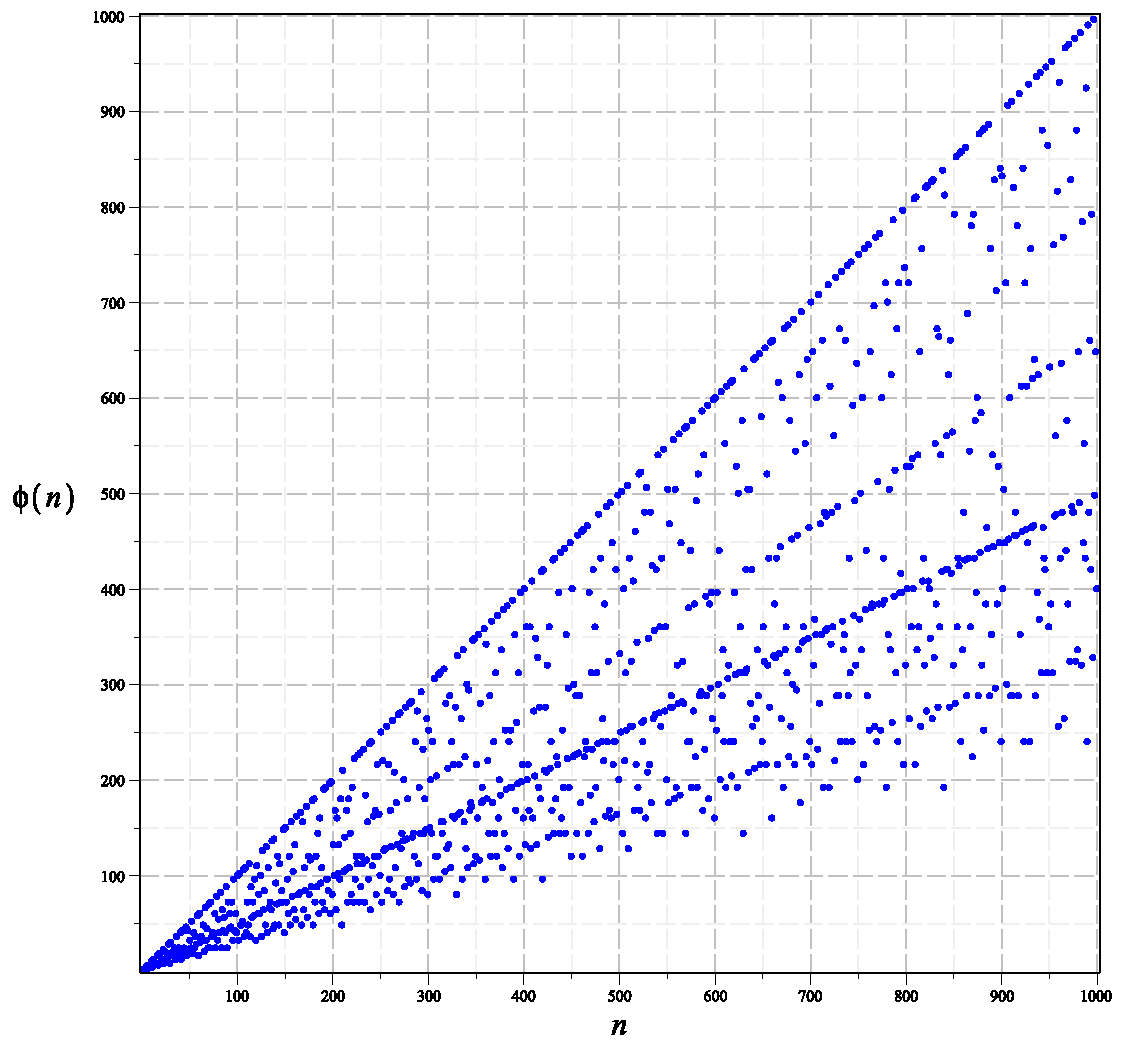
\includegraphics[width=10cm,keepaspectratio]{content/totient.pdf} \\
\vspace*{1cm}
\footnotesize{\url{\homepage}} \\

\vfill
\vspace*{1.5cm}
\begin{flushright}
{\footnotesize Stand: \today}
\end{flushright}
\end{center}
\end{titlepage}							% Titelseite ausgeben
\section*{Vorwort}
\label{sec:preface}
	Der vorliegende Text ist eine Zusammenfassung zur Vorlesung Elementare Zahlentheorie, gelesen von Prof. Dr. Falko Lorenz an der WWU Münster im Wintersemester 2014/2015. Der Inhalt entspricht weitestgehend dem Skript, welches auf der Vorlesungswebsite bereitsgestellt wird, jedoch wird auf Beweise weitestgehend verzichtet. Dieses Werk ist keine Eigenleistung des Autors und wird nicht vom Dozenten der Veranstaltung korrekturgelesen. Für die Korrektheit des Inhalts wird daher keinerlei Garantie übernommen. Bemerkungen, Korrekturen und Ergänzungen kann man folgenderweise loswerden:
	\begin{itemize}
		\item persönlich durch Überreichen von Notizen oder per E-Mail
		\item durch Abändern der entsprechenden TeX-Dateien und Versand per E-Mail an mich
		\item direktes Mitarbeiten via GitHub. Dieses Skript befindet sich im \texttt{latex-wwu}-Repository von Jannes Bantje:
		\begin{center}
			\url{https://github.com/JaMeZ-B/latex-wwu}
		\end{center}
	\end{itemize}

\subsection*{Literatur}
\label{sub:lit}
\begin{itemize}
	\item F. Ischebeck: \href{http://wwwmath.uni-muenster.de/u/ischebeck/}{Einladung zur Zahlentheorie}
	\item R. Remmert, P. Ullrich: \href{http://link.springer.com/book/10.1007/978-3-7643-7731-1}{Elementare Zahlentheorie}
	\item A. Scholz, B. Schöneberg: Einführung in die Zahlentheorie
	\item K. Halupczok: \href{http://wwwmath.uni-muenster.de/u/karin.halupczok/ElZthSS2009Skript.pdf}{Skript zur Elementaren Zahlentheorie}
\end{itemize}

\subsection*{Vorlesungswebsite}
\label{sub:link}
Das vollständige Skript des Dozenten sowie weiteres Material findet man unter folgendem Link:
\begin{center}
	\url{\homepage}
\end{center}

\subsection*{Titelbild}
\label{sub:titlepic}
Plot der Eulerschen $\varphi$-Funktion für $1 \leq n \leq 1000$, erstellt mit Maple. Zugehöriges Maple-Worksheet befindet sich im Git-Repository (siehe oben).

\vfill
\begin{flushright}
	Phil Steinhorst \\
	p.st@wwu.de
\end{flushright}
\newpage
\tableofcontents
\newpage											% Inhaltsverzeichnis ausgeben
\setcounter{section}{-1}
\section{Motivation und Einführung}
\label{sec:para0}

\nextlecture
\subsection*{Kryptologie}
	Die \textbf{Kryptologie} besteht aus den folgenden beiden Gebieten: \marginnote{[1]} 
	\begin{description}
		\item[Kryptographie:] Studium mathematischer Techniken zur Verschlüsselung von Informationen oder geheimen Nachrichten und dem Schutz von Daten.
		\item[Kryptoanalyse:] Beschreibung der Rückgewinnung von Informationen aus verschlüsselten Texten, der Entschlüsselung.
	\end{description}
Oft meint man mit "Kryptographie" die Kryptologie. \\

Früher wurde die Kryptographie vor allem im militärischen oder diplomatischen Sektor verwendet, heutzutage steht in unserer vernetzten Welt vor allem auch der praktische Nutzen im Alltag im Vordergrund: im Internet einkaufen, Online-Banking, persönliche Daten geheimhalten bzw. Datenschutz, Nachrichten und Dokumente digital unterschreiben etc. Das Internet liefert schnelle Informationswege über öffentliche Kanäle, die leicht abgehört werden können, sodass die Verschlüsselung schützenswerter Daten unumgänglich wird. Auch die Möglichkeit zur Signierung wird nötig, weil sehr leicht Absenderangaben gefälscht werden können. Eventuell nicht abhörsichere Kanäle können außer dem Internet aber auch Briefe, Radio, Boten, etc. sein. \\

Bei der \textbf{symmetrischen Verschlüsselung} von Daten gibt es einen Sender $S$ und einen Empfänger $E$, die sich beide auf einen gemeinsamen Schlüssel geeinigt haben, der zum Ver- und Entschlüsseln dient. Beim \Index{Caesar-Code} z.B. ist dies die Vereinbarung, jeden Buchstaben durch den dritten nachfolgenden im Alphabet zu ersetzen, also $A \mapsto D, B \mapsto E, C \mapsto F$, usw. Die Entschlüsselung ist klar. Derartige \textbf{monoalphabetische Chiffrierungen}, bei der jeder Buchstabe des Alphabets stets durch denselben Geheimtextbuchstaben chiffriert wird, sind durch Häufigkeitsanalysen durch einen Angreifer, der die verschlüsselten Nachrichten abhört, sehr leicht zu entschlüsseln. Übrigens gibt es auch heutzutage PDF-Verschlüsselungsprogramme, die so arbeiten! 

In dieser Vorlesung behandeln wir die heutzutage gängigen modernen Methoden, die als sicher gelten. Worauf diese starke Sicherheit beruht, hat mathematische Gründe, die wir besprechen möchten. Vor allem interessiert uns, wie und welche Mathematik in die Kryptologie kommt, sodass wir deren Verfahren verstehen können. \\

Die Anwendungen erfordern die Lösung folgender Probleme bei symmetrischen Verschlüsselungsverfahren:
\begin{itemize}
	\item Schlüsselaustausch über öffentliche Kanäle (\textbf{öffentliche Schlüssel})
	\item Verschlüsselung ohne vorherigen Schlüsselaustausch (mit \textbf{geheimen Schlüsseln}, die nicht versendet werden)
	\item Digitale Signierung und Autentifizierung
\end{itemize}
Dies können \textbf{asymmetrische Verfahren} leisten (auch \textbf{Public Key-Kryptographie} genannt) und gehen zurück auf Ideen von Diffie\footnote{Whitfield Diffie, \url{http://de.wikipedia.org/wiki/Whitfield_Diffie}} und Hellman\footnote{Martin Hellman, \url{http://de.wikipedia.org/wiki/Martin_Hellman}} aus den 70er Jahren: \\

Jeder Nutzer eines Kommunikationskanals hat einen privaten Schlüssel, den er geheim hält und niemand sonst kennt, sowie einen öffentlichen Schlüssel, den jeder einsehen kann. Eine Nachricht wird dann unter Ausnutzung einer Funktion $x \mapsto f(x)$ verschlüsselt, die zwar leicht zu berechnen, aber praktisch nur mit Kenntnis des privaten Schlüssels des rechtmäßigen Empfängers entschlüsselt werden kann. Der Sender der Nachricht wird dafür den öffentlichen Schlüssel des Empfängers zur Verschlüsselung benutzen. Eine derartige Funktion heißt \Index{Einwegfunktion}.

\minisec{Beispiele}
\begin{itemize}
	\item \Index{RSA-Verfahren}: $(p,q) \mapsto p \cdot q$ mit $p,q$ prim.
	\item \Index{ECC-Verfahren}: $x \mapsto mx$ in einer Gruppe auf einer elliptischen Kurve.
\end{itemize}

In einem ersten Teil der Vorlesung stellen wir gängige Verfahren dar, die leicht mit dem Zahlring $\ZZ$ und Strukturen darin realisiert werden können. Dabei werden wir nur einige Hilfsmittel der elementaren Zahlentheorie entwickeln und dafür heranziehen. In einem zweiten Teil studieren wir die Eigenschaften elliptischer Kurven als interessante geometrische und arithmetische Objekte, die sich in der Praxis der Kryptographie als nützlich erwiesen haben. Wir besprechen dann auch die Sicherheit und Implementierung dieser Verfahren und vergleichen sie miteinander.

\subsection*{Elliptische Kurven}
Was sind elliptische Kurven? Jedenfalls sind elliptische Kurven \textbf{keine} Ellipsen. Ellipsen lassen sich durch Gleichungen der Form
\[ \enbrace*{\frac{x}{a}}^2 + \enbrace*{\frac{y}{b}}^2 = 1 \text{ mit } a,b \in \RR \setminus \setnull \]
beschreiben. Durch die Parametrisierung $x(t) = a \cdot \cos(t), y(t) = b \cdot \sin(t)$ ergibt sich für die Bogenlänge der Ellipse ein elliptisches Integral zweiter Art, nämlich
\[ \int_{0}^{2\pi} \sqrt{ \enbrace*{\frac{dx(t)}{dt}}^2 + \enbrace*{\frac{dy(t)}{dt}}^2 } dt = 4 \int_{0}^{2\pi} \sqrt{ a^2 \cos^2(t) + b^2 \cdot \sin^2 (t)} dt \]
Im Allgemeinen lässt sich dies nicht elementar integrieren (außer natürlich, falls $a = b$, d.h. ein Kreis vorliegt). Mit Hilfe von elliptischen Kurven findet man jedoch nicht-elementare Stammfunktionen für diese Integrale\linebreak ($\Rightarrow$ Funktionentheorie). Aufgrund dieses Zusammenhangs haben elliptische Kurven ihren Namen, sie haben ansonsten nichts mit Ellipsen zutun. \\

Was sind nun elliptische Kurven? Es sind "abelsche Varietäten der Dimension 1". Elliptische Kurven sind spezielle algebraische Kurven über einem Körper $k$. Es handelt sich dabei um glatte kubische Kurven, deren definierende algebraische Gleichung sich meist in die Form
\[ E \colon y^2 = x^3 + ax + b \text{ mit } a,b \in k \]
bringen lässt. Als Punktmenge haben wir dafür
\[ E(k) := \{ (x,y) \in k^2 : y^2 = x^3 + ax + b\} \cup \{ \oh \}, \]
die Kurve hängt nur von $a,b$ ab. Die Rolle des zusätzlichen so genannten "unendlich fernen Punkts" $\oh$ werden wir dabei noch näher beleuchten. \\

Zwei typische Beispiele für elliptische Kurven:
\begin{enumerate}[1)]
	\item $E_1\colon y^2 = x^3 + 17$, hier liegen sogar Punkte mit ganzzahligen Koordinaten auf $E_1$, nämlich $(-2,3), (-1,4), (2,5)$. Die Kurve besteht aus einer Zusammenhangskomponente.
	\item $E_2 \colon y^2 = x^3 + ax + b$, wenn $f(x) = x^3 + ax + b$ drei verschiedene Nullstellen hat, z.B. $a = -3, b= -1$. Die Kurve besteht dann aus zwei Zusammenhangskomponenten.
\end{enumerate}

\begin{figure}[h!]
	\centering
	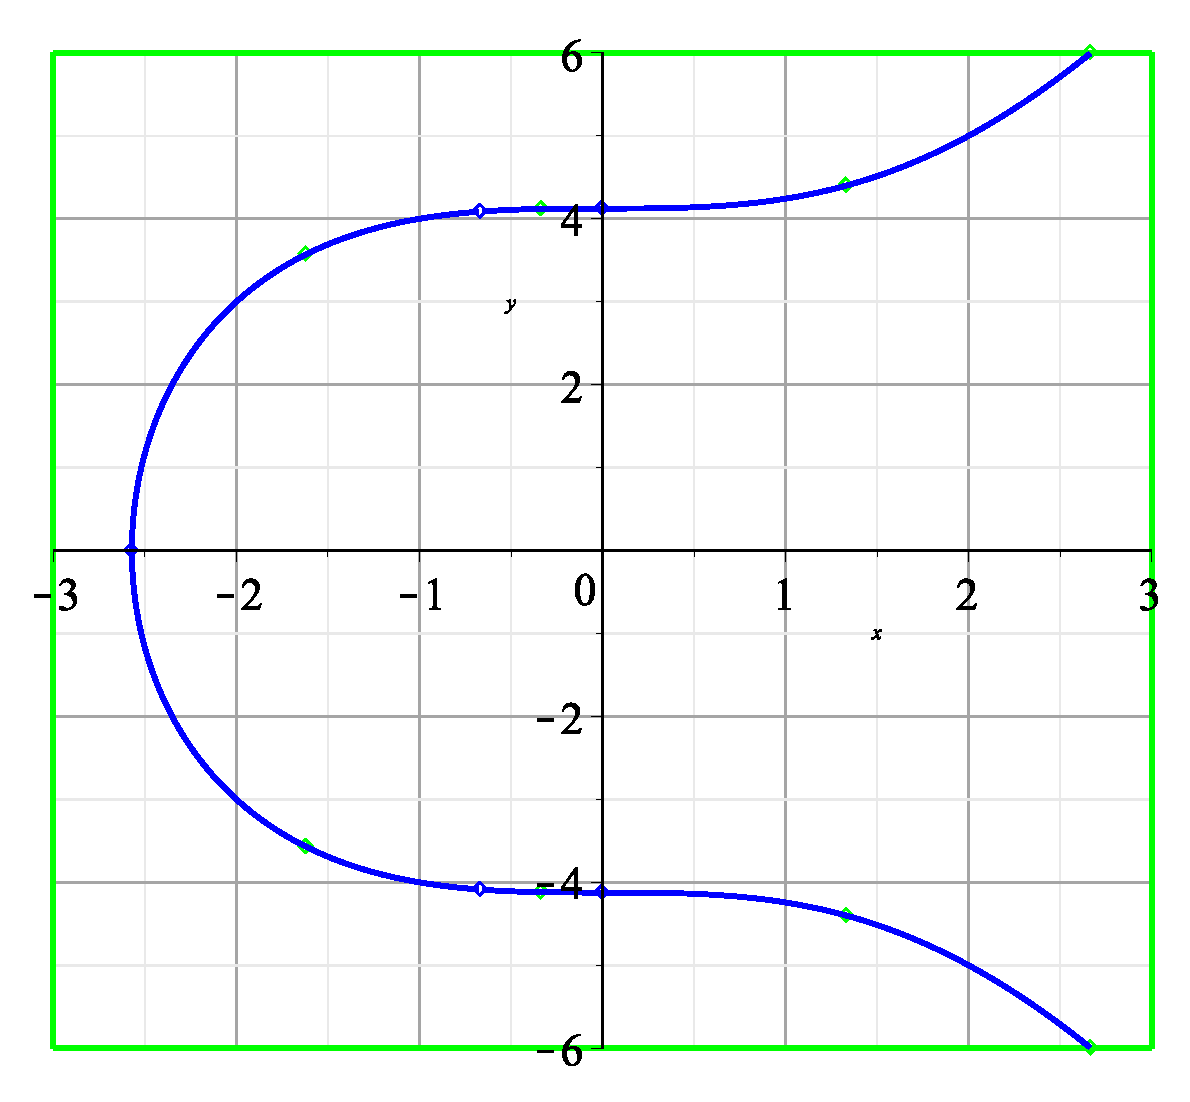
\includegraphics[scale=.3]{img/curve_0_1.eps} \hspace{2cm}
	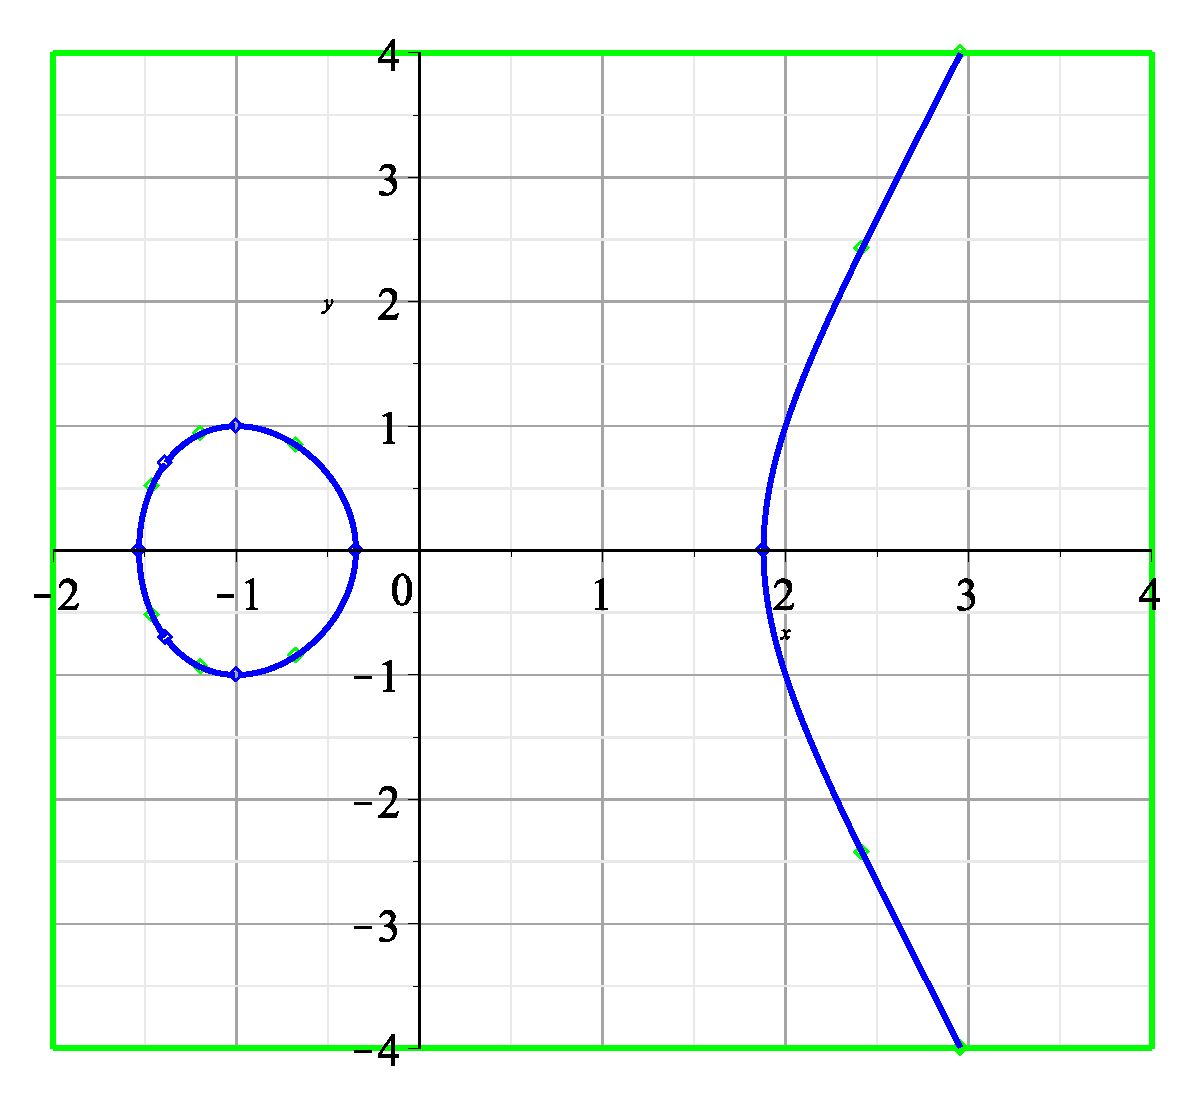
\includegraphics[scale=.3]{img/curve_0_2.eps}
	\caption{Die Kurven $E_1$ (links) und $E_2$ (rechts).}
\end{figure}
%\begin{figure}[h]
%	\centering
%	\begin{tikzpicture}
%	\begin{axis}[
%		scale only axis,
%		xlabel=$x$,
%		ylabel=$y$,
%		grid=major,
%		axis lines=middle,
%		inner axis line style={=>},
%		ymin = -5,
%		ymax = 5,
%		xmin = -3,
%		xmax = 3,
%		xtick={-3,-2,...,3},
%		ytick={-5,-4,...,5}
%	]
%	\addplot[color=red, thick, domain=-2.57128:3, samples=100] {(x^3+17)^(1/2)};
%	\addplot[color=red, thick, domain=-2.57128:3, samples=100] {-(x^3+17)^(1/2)};
%	\end{axis}
%	\end{tikzpicture} \hspace{2cm}
%	\begin{tikzpicture}
%	\begin{axis}[
%		scale only axis,
%		xlabel=$x$,
%		ylabel=$y$,
%		grid=major,
%		axis lines=middle,
%		inner axis line style={=>},
%		ymin = -5,
%		ymax = 5,
%		xmin = -3,
%		xmax = 3,
%		xtick={-3,-2,...,3},
%		ytick={-5,-4,...,5}
%	]
%	\addplot[color=red, thick, domain=-1.53208888:-0.347296, samples=100,unbounded coords=jump] {(x^3-3*x-1)^(1/2)};
%	\end{axis}
%	\end{tikzpicture}
%\end{figure}

\minisec{Bemerkung}
	Die kubischen Kurven $C_1\colon y^2 = x^3 - 3x +2$ und $C_2\colon y^2 = x^3$ z. B. sind jedoch keine elliptischen Kurven, weil diese nicht glatt sind. \\

\begin{figure}[H]
	\centering
	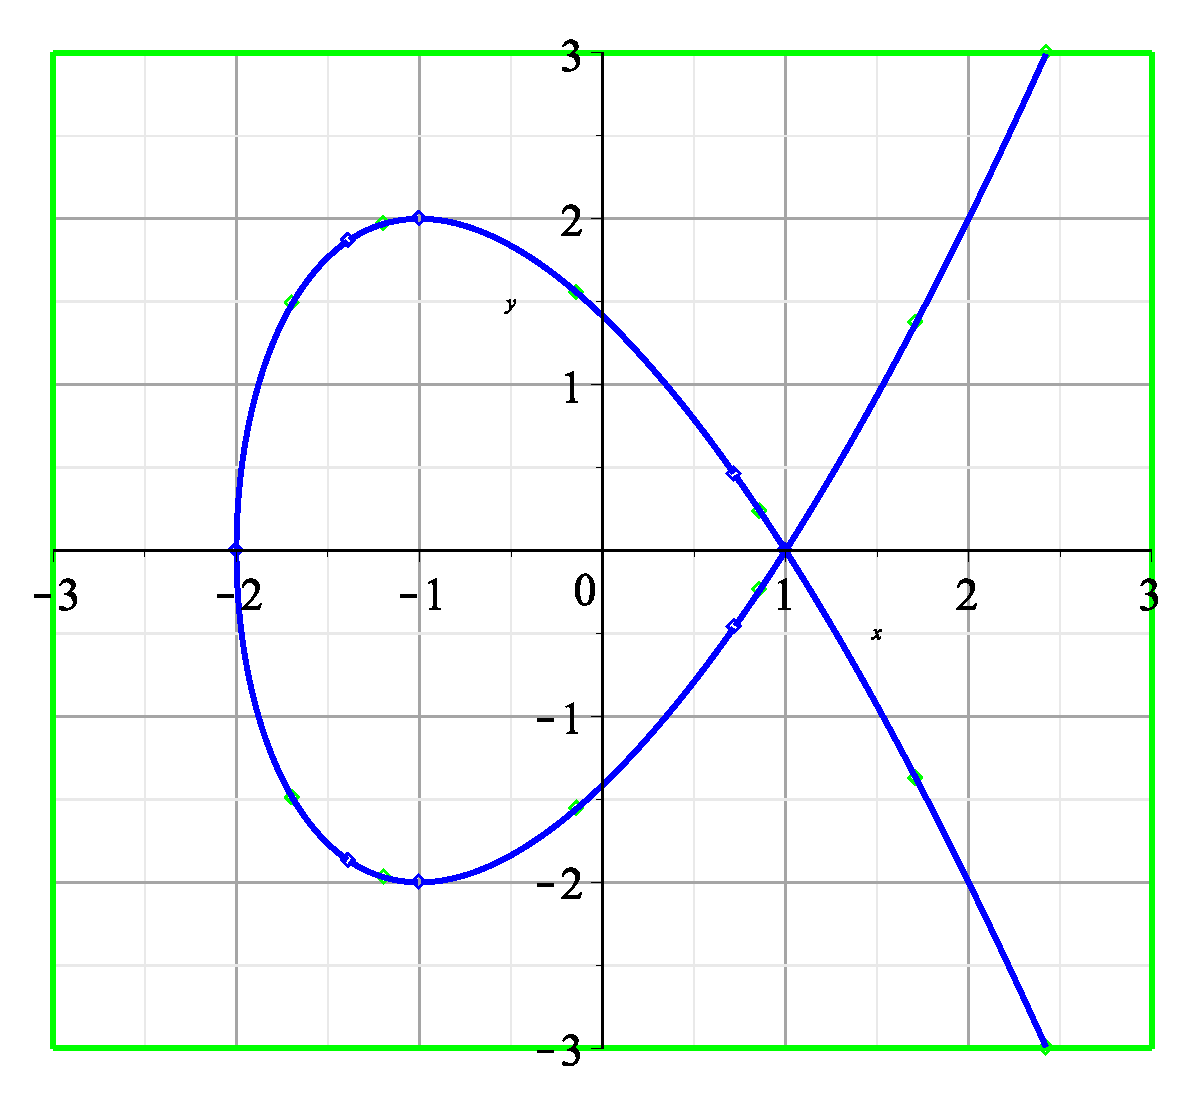
\includegraphics[scale=.3]{img/curve_0_3.eps} \hspace{2cm}
	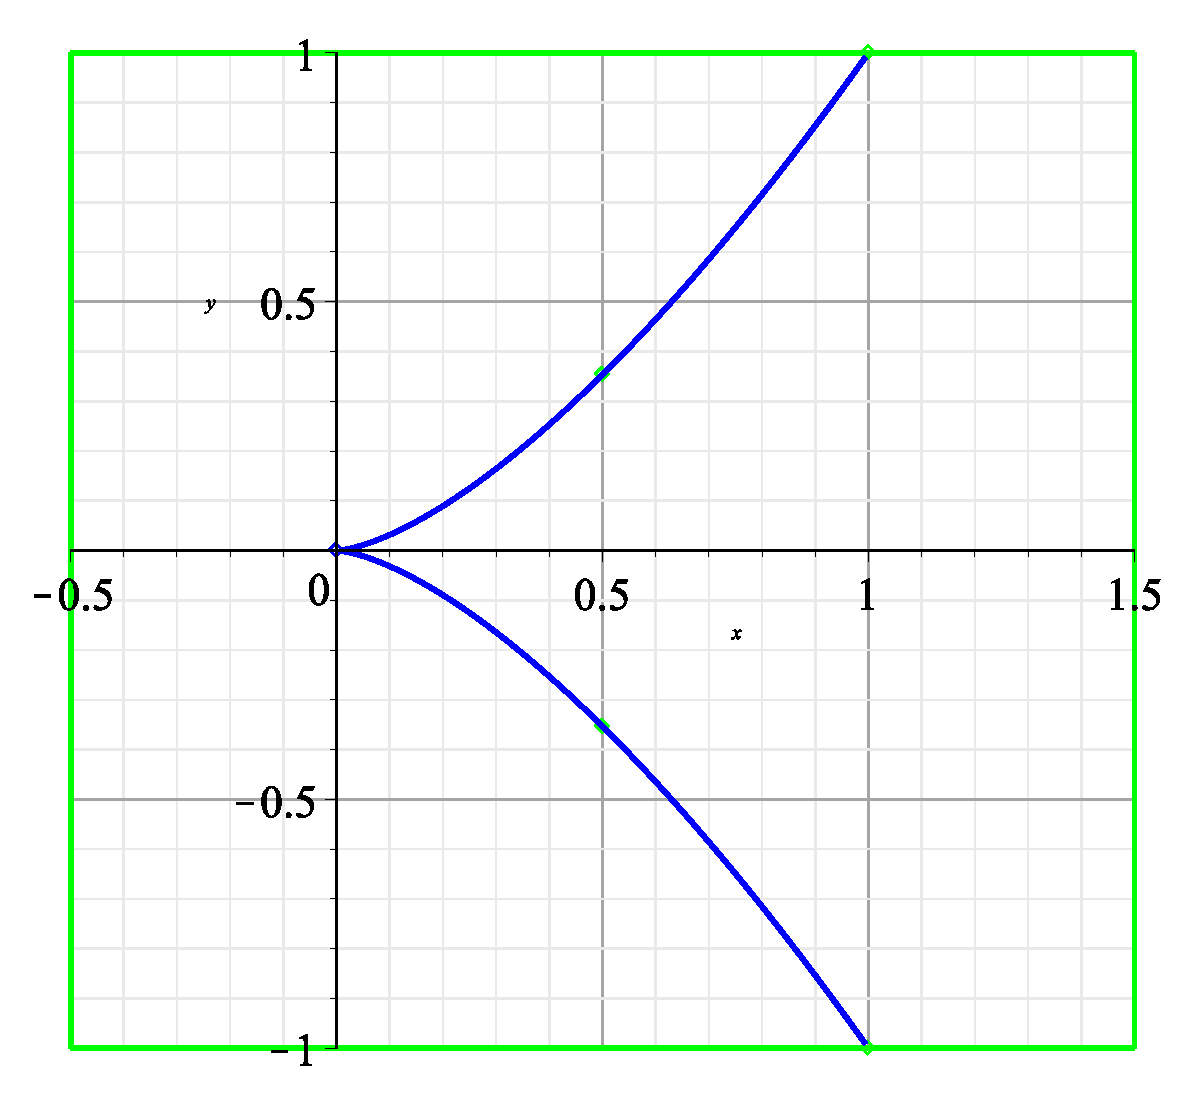
\includegraphics[scale=.3]{img/curve_0_4.eps}
	\caption{Die Kurven $C_1$ (links) und $C_2$ (rechts). $C_1$ ist nicht glatt im Punkt $(1,1)$, $C_2$ nicht im Punkt $(0,0)$.}
	\label{fig:bsp}
\end{figure}

Für die Kryptographie sind elliptische Kurven interessant, weil sich eine Verknüpfung auf ihrer Punktemenge definieren lässt, mit der diese zu einer Gruppe wird. Dabei gerade auch endliche Körper $k$ zuzulassen, macht diese Verknüpfung auf Rechenmaschinen realisierbar. Die Sicherheit der darauf beruhenden elliptic curve cryptography (ECC) beruht darauf, dass das Problem des diskreten Logarithmus auf einer elliptischen Kurve $E$, nämlich die Umkehrung der Funktion $P \mapsto mP$ für $m \in \NN$ fest, nach heutigem Wissensstand rechnerisch im Allgemeinen extrem schwer realisierbar ist.
\newpage
\section{Fundamentalsatz der elementaren Arithmetik}
\label{sec:para1}

\minisec{Terminologie}
	Sei $R$ ein kommutativer Ring mit $1 \neq 0$. $R$ heißt \Index{Integritätsring} bzw. \bet{nullteilerfrei}, wenn gilt: \index{Nullteiler} \marginnote{14.10.}
	\[ a \cdot b = 0 \quad \Rightarrow \quad a = 0 \text{ oder } b = 0.\]

\begin{bsp} \label{bsp_integritaetsringe}
	\begin{itemize}
		\item $\ZZ$
		\item $\ZZ[\sqrt{2}] := \{a + b\sqrt{2} : a,b \in \ZZ \} \subseteq \RR$ \\
			$\ZZ[i] := \{a + bi : a,b \in \ZZ\} \subseteq \CC$ \\
			$\ZZ[\sqrt{-5}] := \dots$
		\item $K[X]$ für $K$ Körper \\
			$\ZZ[X]$
		\item $K$ Körper
		\item $\CC \sprod{z} := \penbrace{\text{konvergente Potenzreihen } \sum\limits_{n=0}^{\infty} a_n z^n}$
		\item Nicht nullteilerfrei ist z.B. $\mathcal{C}[0,1] := \{f \colon [0,1] \rightarrow \RR \text{ stetig} \}$
	\end{itemize}
\end{bsp}

\begin{defn}[Teilbarkeit] \label{def_1.1}
	Seien $a,b \in R$. $a$ heißt ein \Index{Teiler} von $b$, wenn ein $q \in R$ existiert mit $b = qa$, und schreiben:
	\[ a | b \]
	Ist $R$ nullteilerfrei und $a \neq 0$, so ist $q$ eindeutig bestimmt.
\end{defn}

\begin{falko}[Triviale Teilbarkeitsregeln] \label{F1.1}
	\begin{enumerate}[(i)]
		\item $a | 0, 1 | a, a | a$
		\item $a | b, b | c \quad \Rightarrow \quad a | c$
		\item $a | b, a | c \quad \Rightarrow \quad a | b+c, a | b-c$
		\item $a_1 | b_1, a_2 | b_2 \quad \Rightarrow \quad a_1 a_2 | b_1 b_2$
		\item $ac | bc \quad \Rightarrow \quad a | b$, falls $c \neq 0$ und $R$ nullteilerfrei.
	\end{enumerate}	
\end{falko}

\begin{defn}[Einheit, assoziiert] \label{def_1.2}
	\begin{enumerate}[(i)]
		\item $e \in R$ heißt eine \Index{Einheit} in $R$, falls $e | 1$ gilt, d.h. falls ein $f \in R$ existiert mit $ef = 1$. $f$ ist eindeutig bestimmt. Wir setzen $e^{-1} := f$ und schreiben auch $\frac{1}{e}$ für $e^{-1}$. \\
		Wir bezeichnen die \Index{Einheitengruppe} von $R$ mit $R^\times := \{x \in R : x \text{ ist Einheit in } R\}$.
		\item $a \in R$ heißt \Index{assoziiert} zu $b \in R$, falls $a | b$ und $b | a$ gilt. Schreibe: $a \assoz b$.
	\end{enumerate}
\end{defn}

\begin{bsp}
	\begin{enumerate}[1)]
		\item Sei $K$ ein Körper, dann ist $K^\times = K \setminus \setnull$. \qquad $\ZZ^\times = \{1,-1\}$, \qquad $K[X]^\times = K^\times$, \\
		$\mathcal{C}[0,1]^\times = \{f \in \mathcal{C}[0,1] : f(x) \neq 0 \text{ für alle } x \in [0,1]\}$, \qquad  $\ZZ[\sqrt{2}]^\times = \{\pm (1+\sqrt{2})^k : k \in \ZZ \}$ \\
		$\ZZ[X]^\times = \{1, -1\}$ \qquad $\CC \sprod{z}^\times = \penbrace*{ \sum a_n z^n \in \CC \sprod{z} : a_0 \neq 0}$
		\item $e \in R^\times \quad \Leftrightarrow \quad e | a$ für jedes $a \in R$.
	\end{enumerate}
\end{bsp}

\begin{falko} \label{F1.2}
	Sei $R$ ein Integritätsring, $a, b \in R$ und $b \neq 0$. Dann gilt:
	\[ a \assoz b \quad \Leftrightarrow \quad \exists e \in R^\times \text{ mit } b = ea \]
\end{falko}

\minisec{Beweis}
	\begin{description}
		\item[\bewrueck] $a | b, e^{-1}b = a, b | a$
		\item[\bewhin] Da $a | b$ und $b | a$, existieren $e, f \in R$, sodass $b = ea$ und $a = fb$. $\Rightarrow b = efb \Rightarrow ef = 1$, da $b \neq 0$ und $R$ nullteilerfrei. \qed
	\end{description}

\setlength{\fboxsep}{10pt}
\setlength{\fboxrule}{3pt}
\begin{center}
	\fbox{\textbf{Ab jetzt ist, wenn nichts anderes gesagt, $R$ ein Integritätsring!}}
\end{center}

\begin{defn}[unzerlegbar, irreduzibel, zusammengesetzt] \label{def_1.3}
	Sei $a \in R \setminus R^\times$. $a$ heißt \Index{unzerlegbar} oder \Index{irreduzibel} in $R$, wenn gilt:
	\[ a = bc \text{ in } R \quad \Rightarrow \quad b \in R^\times \text{ oder } c \in R^\times. \]
	Andernfalls heißt $a$ \bet{zerlegbar}, \bet{zusammengesetzt} oder \bet{reduzibel}.
\end{defn}

\minisec{Bemerkung}
	$a$ unzerlegbar $\quad \Leftrightarrow \quad $ jeder Teiler von $a$ ist Einheit oder assoziiert zu $a$ \\
	$a$ zerlegbar $\quad \Leftrightarrow \quad a$ hat echten Teiler, d.h. einen Teiler, der weder eine Einheit ist noch assoziiert zu $a$

\setcounter{countdef}{2}
\begin{defn}[Primzahl] \label{def_1.3'}
	Ein $p \in \ZZ$ heißt \Index{Primzahl}, wenn $p \in \NN$ und $p$ unzerlegbar in $\ZZ$. Wir beziechnen mit $\PP$ die Menge der Primzahlen von $\ZZ$. $a$ unzerlegbar in $\ZZ \Leftrightarrow a = p$ oder $a = -p$ mit $p \in \PP$.
\end{defn}

\minisec{Bemerkung}
	$a \in \ZZ$ sei zerlegbar, $a \neq 0$. Dann gibt es eine Primzahl $p$ mit $p | a$ und $p \leq \sqrt{|a|}$.

\begin{defn}[Zerlegung in unzerlegbare Faktoren] \label{def_1.4}
	Wir sagen, $a \in R$ besitzt in $R$ eine \Index{Zerlegung in unzerlegbare Faktoren}, wenn
	\begin{equation}
	\begin{aligned}
		a = ep_1p_2\dots p_r \text{ mit } e \in R^\times \text{ und } p_1,\dots,p_r \text{ unzerlegbar} \label{eq_def_1.4}
	\end{aligned}
	\end{equation}
	\eqref{eq_def_1.4} heißt eine Zerlegung von $a$ in unzerlegbare Faktoren. Auch $r = 0$ ist erlaubt.
\end{defn}

\begin{falko} \label{F1.3}
	In $\ZZ$ besitzt jedes $a \neq 0$ eine Zerlegung in unzerlegbare Faktoren.
\end{falko}	

\setcounter{countfalko}{2}
\begin{falko} \label{F1.3'}
	Jede natürliche Zahl $a > 1$ besitzt eine Zerlegung $a = p_1p_2 \dots p_r$ mit Primzahlen $p_1,\dots,p_r$ und $r \geq 1$.
\end{falko}

\minisec{Bemerkung}
	\begin{enumerate}[1)]
		\item Die Aussage F1.3 gilt auch für die Beispiele zu Beginn, mit Ausnahme von $\mathcal{C}[0,1]$.
		\item Sei $R$ ein Integritätsring, der die \Index{Teilbarkeitsbedingung für Hauptideale} erfüllt, so besitzt jedes $a \neq 0$ aus $R$ eine Zerlegung in unzerlegbare Faktoren.
		\item Primzahlen sind die multiplikativen Bausteine (Atome) von $\NN$.
		\item Im Beispiel $\CC\sprod{z}$ von oben gibt es (bis auf Assoziiertheit) nur das einzige unzerlegbare Element $z$. Dieses ist ein \Index{Primelement} (der Begriff folgt weiter unten).
	\end{enumerate}
	
\begin{satz}[Existenz unendlich vieler Primzahlen] \label{satz_1.1}
	Es gibt unendlich viele Primzahlen.
\end{satz}

\textbf{Bemerkungen} \\
	Es sei $p_1,p_2,\dots$ die aufsteigend sortierte Folge der Primzahlen.
	\begin{enumerate}[1)]
		\item $a_n := p_1p_2\dots p_n +1$ ist Primzahl für $n \leq 5$, aber z.B. nicht für $n = 6$. Unklar ist, ob unendlich viele $a_n$ Primzahlen oder keine Primzahlen sind.
		\item Für $x \in \RR_{>0}$ definieren wir:
		\[ \pi(x) := \# \penbrace{p \in \PP : p \leq x}\]
	\end{enumerate}

\minisec{Primzahlsatz (Gauß, Legendre)}
	\begin{equation}
		\pi(x) \sim \frac{x}{\log x}, \text{ d.h. } \lim\limits_{x \rightarrow \infty} \frac{\pi(x)}{x / \log x} = 1 \label{eq_primzahlsatz1}
	\end{equation}
	\begin{equation}
		\pi(x) \sim \int_{2}^{x} \frac{1}{\log t} dt =: \li(x) \label{eq_primzahlsatz_2}
	\end{equation}
	\begin{equation}
	\pi(x) > \frac{x}{\log x} \text{ für alle } x \geq 17 \label{eq_primzahlsatz_3}
	\end{equation}
	\begin{equation}
	\pi(n) > \frac{n}{\log n} \text{ für alle } n \in \NN, n \geq 11 \label{eq_primzahlsatz_4}
	\end{equation}
	
\begin{defn}[eindeutige Zerlegung] \label{def_1.5}
	Sei $R$ ein kommutativer Ring mit $1 \neq 0$. Wir sagen, $a \in R \setminus \setnull$ hat eine \bet{eindeutige} \Index{Zerlegung in unzerlegbare Faktoren}, wenn $a$ eine Zerlegung
	\[ a = ep_1p_2 \dots p_r \]
	in unzerlegbare Faktoren besitzt und eine solche im folgendem Sinne eindeutig ist: Ist auch
	\[ a = e'p_1'p_2'\dots p'_{r'} \]
	eine solche Zerlegung, so gilt $r = r'$ und nach Umnummerierung $p_i' \assoz p_i$ für alle $1 \leq i \leq r$.
\end{defn}

\begin{falko}\label{F1.4}
	In dem Integritätsring $R$ besitze jedes Element $a \neq 0$ eine Zerlegung in unzerlegbare Faktoren. Dann sind äquivalent: \begin{enumerate}[(i)]
		\item Jedes $a \neq 0$ aus $R$ hat eindeutige Zerlegung in unzerlegbare Faktoren.
		\item Ist $p$ unzerlegbar, so gilt: $p | ab \Rightarrow p | a$ oder $p | b$.
	\end{enumerate}
\end{falko}

\begin{defn}[Primelement] \label{def_1.6}
	Sei $R$ ein kommutativer Ring mit $1 \neq 0$. Ein $p \in R\setminus R^\times$ heißt \Index{Primelement} von $R$, wenn für alle $a, b \in R$ gilt:
	\begin{equation}
		p | ab \quad \Leftrightarrow \quad p | a \text{ oder } p | b \label{eq_def_1.6}
	\end{equation}
\end{defn}

\minisec{Bemerkung}
	\begin{enumerate}[1)]
		\item $0$ ist Primelement in $R \Leftrightarrow R$ ist Integritätsring
		\item In einem Integritätsring $R$ gilt: Jedes Primelement $p \neq 0$ ist unzerlegbar.
	\end{enumerate}

\begin{lemma}
	Seien $a, b \in \NN$. Sei $m = \kgV(a,b) \in \NN$. Dann gilt:
	\[ a|c \text{ und } b|c \quad \Rightarrow \quad m | c \]
	$m$ ist also auch minimal bzgl. der Teilbarkeitsrelation $|$.
\end{lemma}

\begin{falko}[Satz von Euklid] \label{F1.5}
	Jede Primzahl $p$ ist ein Primelement von $\ZZ$, d.h. es gilt stets \eqref{eq_def_1.6}. (Das gleiche gilt für $-p$, also für jedes unzerlegbare Element von $\ZZ$.) \index{Satz von Euklid}
\end{falko}

\minisec{Fundamentalsatz der elementaren Arithmetik}
	In $\ZZ$ hat jedes $a \neq 0$ eine eindeutige Zerlegung in unzerlegbare Faktoren. \index{Fundamentalsatz der elementaren Arithmetik}

\minisec{Bemerkung}
	Eindeutige Zerlegung in unzerlegbare Faktoren hat man zum Beispiel auch für die Ringe $\ZZ[\sqrt{2}], \ZZ[i], K[X]$ und $K$ für $K$ Körper, $\ZZ[X]$ und $\CC\sprod{z}$, nicht aber für $\ZZ[\sqrt{-5}]$:
	\[ 3 \cdot 3 = 9 = (2+ \sqrt{-5})(2 - \sqrt{-5}) \]
	Dies sind zwei wesentlich verschiedene Zerlegungen in unzerlegbare Faktoren.

\begin{defn}[Exponent] \label{def_1.7}
	Sei $p$ eine Primzahl und $a \in \ZZ \setminus \setnull$. Dann heißt
	\[ w_p(a) :=\max\{k \in \NN_0 : p^k |a \} \]
	der \Index{Exponent} von $p$ in $a$. Wir setzen $w_p(0) := \infty$.
\end{defn}

\begin{falko}[Eigenschaften der Exponentfunktion] \label{F1.6}
	Die Funktion $w_p \colon \ZZ \rightarrow \NN_0 \cup \{\infty\}$ hat folgende Eigenschaften:
	\begin{enumerate}[(i)]
		\item $w_p(a+b) \geq \min(w_p(a),w_p(b))$ und Gleichheit, falls $w_p(a) \neq w_p(b)$.
		\item $w_p(ab) = w_p(a) + w_p(b)$
	\end{enumerate}
\end{falko}

\begin{satz}[Fundamentalsatz der elementaren Arithmetik] \label{satz_1.2}
	Für jedes $a \in \ZZ \setminus \setnull$ gilt $w_p(a) > 0$ nur für endlich viele $p$. Es ist
	\begin{equation}
		a = \sgn(a) \cdot \prod\limits_p^{} p^{w_p(a)} \label{eq_satz_1.2}
	\end{equation}
\end{satz}

\minisec{Bemerkung}
	\begin{enumerate}[1)]
		\item $w_p$ lässt sich eindeutig zu einer Abbildung $w_p \colon \QQ \rightarrow \ZZ \cup \{\infty\}$ fortsetzen, sodass (ii) für alle $a,b \in \QQ$ gilt. Es gilt dann auch (i). Für $a \in \QQ \setminus \setnull$ ist $w_p(a) \neq 0$ nur für endlich viele $p$, und die Formel \eqref{eq_satz_1.2} gilt entsprechend.  Ferner gilt: $a \in \ZZ \Leftrightarrow w_p(a) \geq 0$ für alle $p$.
		\item Sei
		\[ \NN_0^{(\PP)} := \{ (e_p)_{p \in \PP} : e_p \in \NN_0, e_p = 0 \text{ für fast alle } p \}. \]
		Nach Satz \ref{satz_1.2} sind $(\NN,\cdot)$ und $(\NN_0^{(\PP)},+)$ zwei zueinander isomorphe Halbgruppen. Nach Bemerkung 1) sind $\QQ^\times$ und $\{1,-1\} \times \ZZ^{(\PP)}$ sogar zwei zueinander isomorphe Gruppen.
	\end{enumerate}
	
\begin{defn}[faktorieller Ring, Vertretersystem für Primelemente] \label{def_1.8}
	Ein Integritätsring $R$ heißt \Index{faktoriell}, wenn jedes $a \in R \setminus \setnull$ eine eindeutige Zerlegung in unzerlegbare Faktoren hat. Man spricht dann auch von eindeutiger Primfaktorzerlegung in $R$. \\
	$P$ heißt \bet{Vertretersystem für die Primelemente $\neq 0$} von $R$, wenn:
	\begin{enumerate}[(1)]
		\item Zu jedem Primelement $q \neq 0$ von $R$ gibt es ein $p \in P$ mit $q \assoz p$. 
		\item Für $p, p' \in P$ mit $p \assoz p'$ gilt $p = p'$, d.h. $p$ in (1) ist eindeutig bestimmt durch $q$.
	\end{enumerate}
	Für $R = \ZZ$ nehme man stets $P = \PP$. Für $K$ Körper und $R = K[X]$ nimmt man $P = \{p \in K[X] : p \text{ irreduzibel und normiert}\}$. \index{Primelement} \index{Vertretersystem}
\end{defn}

\begin{falko} \label{F1.7}
	Sei $R$ faktoriell und $P$ ein Vertretersystem für Primelemente. Es gibt zu jedem $p \in P$ eine Funktion $w_p \colon R \rightarrow \NN_0 \cup \{\infty\}$ mit den Eigenschaften (i) und (ii) aus F\ref{F1.6}, sodass gilt: \begin{enumerate}[a)]
		\item Für jedes $a \in R \setminus \setnull$ ist $w_p(a) > 0$ nur für endlich viele $p \in P$.
		\item Für jedes $a \in R \setminus \setnull$ gilt
		\begin{equation}
			a = e \prod\limits_{p \in P}^{} p^{w_p(a)} \label{eq_F1.7}
		\end{equation}
		mit eindeutigem $e \in \RR^\times$.
	\end{enumerate}
\end{falko}

\begin{defn}[ggT und kgV] \label{def_1.9}
	Sei $R$ ein kommutativer Ring mit $1 \neq 0$. Gegeben $a_1, \dots, a_n \in R$.
	\begin{enumerate}[a)]
		\item Ein $d \in R$ heißt ein \Index{größter gemeinsamer Teiler} (ggT) von $a_1,\dots,a_n$, falls:
		\begin{center}
			1. \quad $d | a_i$ für alle $i$ \hspace{3cm} 2. \quad $t | a_i$ für alle $i \Rightarrow t | d$
		\end{center}
		\item Ein $m \in R$ heißt ein \Index{kleinstes gemeinsames Vielfaches} (kgV) von $a_1,\dots,a_n$, falls:
		\begin{center}
			1. \quad $a_i | m$ für alle $i$ \hspace{3cm} 2. \quad $a_i | c$ für alle $i \Rightarrow m | c$
		\end{center}
	\end{enumerate}
\end{defn}

\minisec{Bemerkung}
	\begin{enumerate}[1)]
		\item $d, d'$ ggT von $a_1, \dots, a_n \Rightarrow d \assoz d'$ und $m, m'$ kgV von $a_1, \dots, a_n \Rightarrow m \assoz m'$
		\item Im Allgemeinen ist die Existenz eines ggT und kgV nicht gesichert. In faktoriellen Ringen existieren sie aber immer, siehe dazu folgende Feststellung.
	\end{enumerate}
\newpage

%\appendix							% Anhang beginnt hier (Nummerierung mit Buchstaben)
\printindex							% Index ausgeben
\subsection*{Liste der Sätze und Definitionen}
\listtheorems{satz}					% listet angegebene Sätze mit Namen und Seitenzahl auf
\end{document}